\documentclass[border=8pt]{standalone}
\usepackage[T1]{fontenc}\usepackage[utf8]{inputenc}
\usepackage{helvet}\renewcommand{\familydefault}{\sfdefault}
\usepackage{tikz,xcolor}
\usetikzlibrary{arrows.meta,positioning,shapes.geometric,shapes.multipart,calc,fit,backgrounds,decorations.markings}
\definecolor{ink}{HTML}{1E1B16}\definecolor{paper}{HTML}{FBF8F2}\definecolor{clay}{HTML}{B5482A}\definecolor{soft}{HTML}{F1E9DA}\definecolor{pine}{HTML}{24402F}
\tikzset{
  every node/.style={font=\small,text=ink},
  >=Stealth, line/.style={draw=ink,line width=0.8pt},
  cls/.style={rectangle split,rectangle split parts=3,draw=ink,line width=0.8pt,fill=soft,align=left,inner xsep=6pt,inner ysep=4pt,
              rectangle split part align={center,left,left},minimum width=3.0cm},
  cls2/.style={rectangle split,rectangle split parts=2,draw=ink,line width=0.8pt,fill=soft,align=left,inner xsep=6pt,inner ysep=4pt,
              rectangle split part align={center,left},minimum width=3.0cm},
  box/.style={rectangle,draw=ink,line width=0.8pt,fill=soft,align=center,inner sep=5pt,minimum height=0.8cm},
  state/.style={rectangle,rounded corners=8pt,draw=ink,line width=0.8pt,fill=soft,align=center,inner sep=6pt,minimum width=2.2cm,minimum height=0.9cm},
  act/.style={rectangle,rounded corners=10pt,draw=ink,line width=0.8pt,fill=soft,align=center,inner sep=5pt,minimum width=2.4cm,minimum height=0.8cm},
  dec/.style={diamond,draw=ink,line width=0.8pt,fill=soft,inner sep=1pt,minimum width=0.9cm,minimum height=0.9cm},
  uc/.style={ellipse,draw=ink,line width=0.8pt,fill=soft,align=center,inner sep=3pt,minimum width=3.2cm,minimum height=1.0cm},
  note/.style={rectangle,draw=ink,line width=0.6pt,fill=yellow!12,align=left,inner sep=4pt,font=\footnotesize},
  lab/.style={font=\footnotesize,fill=paper,inner sep=1.5pt},
  err/.style={},
}
\newcommand{\actor}[3]{% x,y,label
  \draw[line width=0.8pt] (#1,#2+0.55) circle (0.17);
  \draw[line width=0.8pt] (#1,#2+0.38)--(#1,#2-0.15) (#1-0.3,#2+0.22)--(#1+0.3,#2+0.22) (#1,#2-0.15)--(#1-0.25,#2-0.6) (#1,#2-0.15)--(#1+0.25,#2-0.6);
  \node[font=\small] at (#1,#2-0.9) {#3};}
\begin{document}
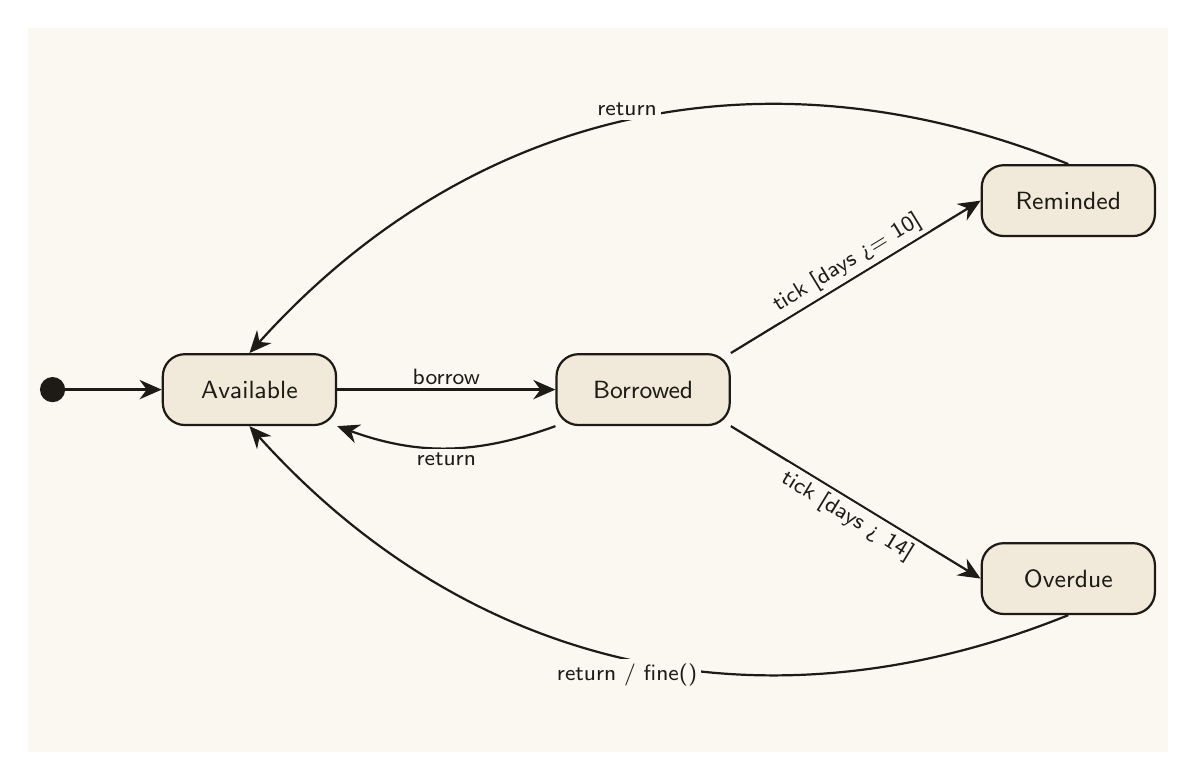
\begin{tikzpicture}[background rectangle/.style={fill=paper},show background rectangle]
\fill[ink] (-1.3,0) circle (0.16);
\node[state] (av) at (1.2,0) {Available};
\node[state] (bo) at (6.2,0) {Borrowed};
\node[state] (re) at (11.6,2.4) {Reminded};
\node[state] (ov) at (11.6,-2.4) {Overdue};
\draw[line,-{Stealth[length=8pt,width=7pt]}] (-1.14,0)--(av.west);
\draw[line,-{Stealth[length=8pt,width=7pt]}] (av.east)--(bo.west) node[midway,above,lab]{borrow};
\draw[line,-{Stealth[length=8pt,width=7pt]}] (bo.south west) to[bend left=20] node[midway,below,lab]{return} (av.south east);
\draw[line,-{Stealth[length=8pt,width=7pt]}] (bo.north east) -- node[above,sloped,lab]{tick [days >= 10]} (re.west);
\draw[line,-{Stealth[length=8pt,width=7pt]}] (bo.south east) -- node[below,sloped,lab]{tick [days > 14]} (ov.west);
\draw[line,-{Stealth[length=8pt,width=7pt]}] (re.north) to[bend right=35] node[above,lab]{return} (av.north);
\draw[line,-{Stealth[length=8pt,width=7pt]}] (ov.south) to[bend left=35] node[below,lab]{return / fine()} (av.south);
\end{tikzpicture}
\end{document}
